\documentclass{beamer}
\usepackage{etex}
\usepackage{lmodern}
\usepackage[english]{babel}
\usepackage[T1]{fontenc}
\usepackage[utf8]{inputenc}
\usepackage{pst-sigsys} 
\usepackage{amsmath,amsfonts,amssymb}
\usepackage{pstricks-add} 
\usepackage{ragged2e}
\usepackage{graphicx}
\usepackage{ulem}
\usepackage{fontawesome}
\setbeamertemplate{navigation symbols}{}  
 
\usetheme{Darmstadt}
\setbeamertemplate{footline}{\insertframenumber/\inserttotalframenumber}
\title{M1 IEAP - BTI/FH/IEMH\\pFIEA02CM : Analyse et Traitement du Signal}
\author{Flavy ROSEREN\\Martin EGIZIANO\\Frank BULOUP}
\institute{Aix Marseille Université\\Institut des Sciences du Mouvement}
\date{}

\setbeamertemplate{footline} 
{  
	\begin{beamercolorbox}[ht=2.5ex,dp=1.125ex,%
      leftskip=.3cm,rightskip=.3cm plus1fil]{title in head/foot}%
      {\usebeamerfont{title in head/foot}\insertshorttitle} \hfill    
      \insertframenumber / \inserttotalframenumber%
    \end{beamercolorbox}%
%     \begin{beamercolorbox}[colsep=1.5pt]{lower separation line foot}
%     \end{beamercolorbox} 
}

\newcounter{exampleBlockCounter}
\setcounter{exampleBlockCounter}{1}

\begin{document} 
 
\begin{frame}[plain] 
	\titlepage 
	\center{
\includegraphics[scale=0.75]{images/by-nc-sa.eps}}
	\vspace{1cm}
	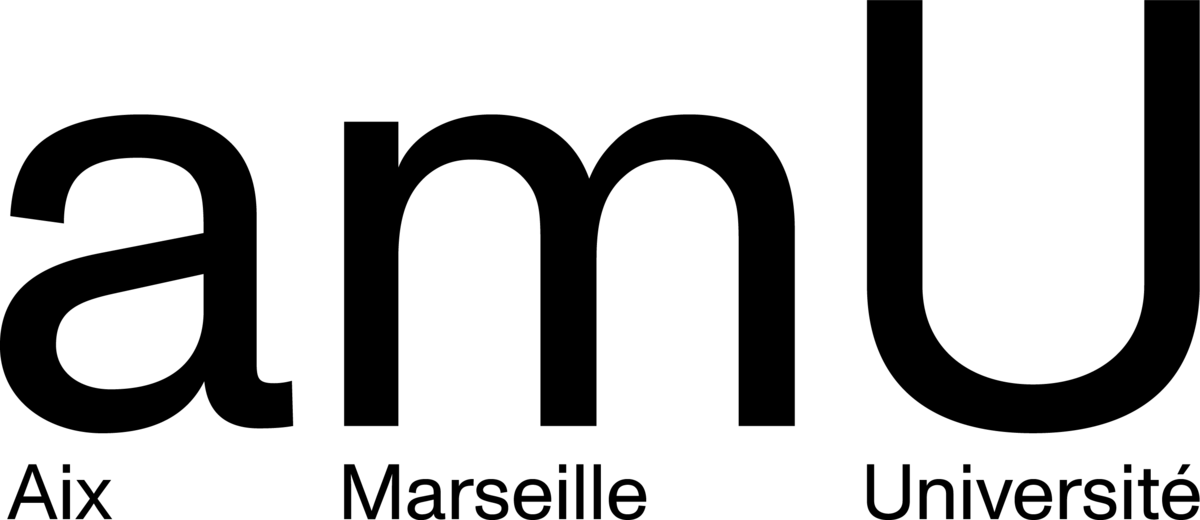
\includegraphics[scale=0.6]{images/LogoAMU.png}\hspace*{2cm}
	
\includegraphics[scale=0.2]{images/LogoCNRS.eps}\hspace*{2cm}
	
\includegraphics[scale=0.1]{images/LogoISM.eps}
\end{frame}

\begin{frame}{Première Partie}
	\tableofcontents
\end{frame}

\section{Signal discret - Aspect fréquentiel}
\subsection{Représentation fréquentielle des signaux}
\begin{frame}
\begin{exampleblock}{Mais dans la majorité des cas pratiques :}
\itemize\justifying
  \item on enregistre des phénomènes transitoires, non
  périodique
  \item les signaux sont discrets, sur ordinateur, issus d'une 
  acquisition de données)
\end{exampleblock} 
\center{\textcolor{red}{À quoi peut donc bien servir la série de Fourier ? =>
TFD}}
\pause
\begin{alertblock}{Transformée de Fourier Discrète (TFD)}
\itemize\justifying
  \item La période $T_0$ correspond à la durée de l'enregistrement plus un
  pas d'échantillonnage : $NT_e$ ($T_e$ étant la période ou le pas
  d'échantillonnage)
  \item La sommation n'est plus continue mais discrète sur tous les échantillons
  acquis
  \item La variable $t$ est discrétisée et se transforme en $nT_e$
  \item $dt$ correspond au pas d'échantillonnage $T_e$
\end{alertblock}
\end{frame}

\subsection{Transformées de Fourier Discrète et Rapide (TFD, TFR)}
\begin{frame}
On obtient alors la Transformée de Fourier Discrète :
\begin{align*}
S(k) = \frac{1}{NT_e}\sum_{n=0}^{N-1}s(nT_e)e^{-2i\pi k \frac{1}{NT_e} nT_e}T_e
\end{align*}
\begin{block}{Transformée de Fourier Discrète (TFD)}
\begin{align*}
S(k) = \frac{1}{N}\sum_{n=0}^{N-1}s(n)e^{-2i\pi \frac{kn}{N}}
\end{align*}
\end{block}
\pause
\begin{block}{Transformée de Fourier Discrète Inverse (TFDI)}
Il existe une transformée inverse
\begin{align*}
s(n) = \sum_{k=0}^{N-1}S(k)e^{2i\pi \frac{kn}{N}}
\end{align*}
\end{block}

\end{frame}

\begin{frame}
\begin{alertblock}{Remarques}
\itemize\justifying
\item Dans la série de Fourier, les fréquences sont des multiples de $f_0$. Dans
la TFD les fréquences sont des multiples de $\frac{F_e}{N}$
\item On dit que $\frac{F_e}{N}$ est la résolution fréquentielle de la TFD
\item Il existe une méthode rapide de calcul des TFD : l'algorithme de
Transformée de Fourier Rapide (Fast Fourier Transform)
\item $\rho(k)$ et $\phi(k)$ se calculent de la même manière que pour la série
de Fourier
\end{alertblock}
\pause
\begin{block}{Autres définitions}
Ces définitions des TFD ne sont pas uniques. Le facteur $\frac{1}{N}$ peut se
trouver dans la transformée inverse
\[
S(k) = \sum_{n=0}^{N-1}s(n)e^{-2i\pi \frac{kn}{N}} \quad s(n) =
\frac{1}{N}\sum_{k=0}^{N-1}S(k)e^{2i\pi \frac{kn}{N}}
\]
\end{block}
\end{frame}

\begin{frame}
\begin{exampleblock}{Exercice FFT Python}
Représenter les spectres des signaux suivants en utilisant les commandes $fft$ et $stem$ de Python :
\begin{itemize}
  \item $s_1(t) = 3$
  \item $s_2(t) = 6sin(2\pi t)$
  \item $s_3(t) = 1 + 2cos(10\pi t) + 4cos(20\pi t + \frac{\pi}{6})$
  \item $s_4(t) = cos(100\pi t) + cos^2(100\pi t)$
\end{itemize}
\end{exampleblock}
\pause
\begin{alertblock}{Remarque importante}
\justifying
La command $fft$ de Python donne un résultat qui fait intervenir le spectre bilatéral où les fréquences négatives doivent être prises en compte.
\end{alertblock}
\end{frame}


\begin{frame}
\begin{exampleblock}{Exercice TFD}
\begin{enumerate}\justifying
	\item Exprimer $\overline{S(k)}$ en fonction de $S(-k)$ lorsque $s(t)$ est un
	signal réel
	\item En déduire les relations liant $\rho(k)$ à $\rho(-k)$ et $\phi(k)$ à
	$\phi(-k)$
	\item Si on a acquis un signal à la fréquence $F_e$, quelle est la fréquence
	maximale observable ?
	\item Dans les expressions précédentes de la TFD, quelle doit-être la
	fréquence maximale ?
	\item Conclusions ?
\end{enumerate}
\end{exampleblock}
\pause
\begin{alertblock}{Représentation bilatérale de la TFD}
\justifying
$S(k)$ possède une certaine symétrie par rapport à l'origine et ne peut contenir
d'énergie à des fréquences supérieures à $\frac{F_e}{2}$. Une 
représentation physiquement cohérente correspond donc
au \textcolor{red}{\textbf{spectre bilatéral}} : le signal comporte de
l'énergie entre $-\frac{F_e}{2}$ et $\frac{F_e}{2}$.
\end{alertblock}
\end{frame}



\begin{frame}
\begin{block}{Spectre de module bilatéral - Fonction paire}
\begin{columns}[t]
	\begin{column}{4cm}
		Ce que donne la TFD
		\begin{figure}
			\psset{unit=0.5cm}	
			\begin{pspicture}[showgrid=false](0,-1)(7,3)
				\psaxeslabels{->}(0,0)(0,0)(7,3){$f$}{$Amplitude$}
				\psstem[style=Stem]{2,.5,1,0}
				\psset{linecolor=red}
				\psstem[style=Stem](4,1){0,1,.5}
				\rput(0,-.5){$0$}
				\psline[linecolor=red](3.5,-.15)(3.5,.15)
				\rput(3.5,-.7){\textcolor{red}{$\frac{F_e}{2}$}}
				\psline[linecolor=red](6.5,-.15)(6.5,.15)
				\rput(6.25,-.7){\textcolor{red}{$F_e$}}
			\end{pspicture}
		\end{figure}
	\end{column}
	\begin{column}{4cm}
		Ce que l'on a en réalité
		\begin{figure}
			\psset{unit=0.5cm}	
			\begin{pspicture}[showgrid=false](-4,-1)(4,3)
				\psaxeslabels{->}(0,0)(-4,0)(4,3){$f$}{$Amplitude$}
				\psstem[style=Stem]{2,.5,1,0}
				\psset{linecolor=red}
				\psstem[style=Stem](-3,1){0,1,.5}
				\rput(0,-.5){$0$}
				\psline[linecolor=red](3.5,-.15)(3.5,.15)
				\rput(3.25,-.7){\textcolor{red}{$\frac{F_e}{2}$}}
				\psline[linecolor=red](-3.5,-.15)(-3.5,.15)
				\rput(-3.5,-.7){\textcolor{red}{$\text{-}\frac{F_e}{2}$}}
			\end{pspicture}
		\end{figure}
	\end{column}
\end{columns}
\end{block}
\begin{block}{Spectre de phase bilatéral - Fonction impaire}
\begin{columns}[t]
	\begin{column}{4cm}
		Ce que donne la TFD
		\begin{figure}
			\psset{unit=0.5cm}	
			\begin{pspicture}[showgrid=false](0,-2)(7,2)
				\psaxeslabels{->}(0,0)(0,-2)(7,2){$f$}{$Phase$}
				\psstem[style=Stem]{0,-.5,-1,-1.5}
				\psset{linecolor=red}
				\psstem[style=Stem](4,1){1.5, 1, .5}
				\rput(.250,-.5){$0$}
				\psline[linecolor=red](3.5,-.15)(3.5,.15)
				\rput(3.5,-.7){\textcolor{red}{$\frac{F_e}{2}$}}
				\psline[linecolor=red](6.5,-.15)(6.5,.15)
				\rput(6.25,-.7){\textcolor{red}{$F_e$}}
			\end{pspicture}
		\end{figure}
	\end{column}
	\begin{column}{4cm}
		Ce que l'on a en réalité
		\begin{figure}
			\psset{unit=0.5cm}	
			\begin{pspicture}[showgrid=false](-4,-2)(4,2)
				\psaxeslabels{->}(0,0)(-4,-2)(4,2){$f$}{$Phase$}
				\psstem[style=Stem]{0,-.5,-1,-1.5}
				\psset{linecolor=red}
				\psstem[style=Stem](-3,1){1.5, 1, .5}
				\rput(.250,-.5){$0$}
				\psline[linecolor=red](3.5,-.15)(3.5,.15)
				\rput(3.5,.7){\textcolor{red}{$\frac{F_e}{2}$}}
				\psline[linecolor=red](-3.5,-.15)(-3.5,.15)
				\rput(-3.5,-.7){\textcolor{red}{$\text{-}\frac{F_e}{2}$}}
			\end{pspicture}
		\end{figure}
	\end{column}
\end{columns}
\end{block}
\end{frame}

\begin{frame}
\begin{exampleblock}{Exercices représentation spectrale bilatérale}
Représenter les spectres bilatéraux des signaux suivants :
\begin{itemize}
  \item $s_1(t) = 3$
  \item $s_2(t) = 6sin(2\pi t)$
  \item $s_3(t) = 1 + 2cos(10\pi t) + 4cos(20\pi t + \frac{\pi}{6})$
  \item $s_4(t) = cos(100\pi t) + cos^2(100\pi t)$
\end{itemize}
\vspace{0.5cm}
Refaire cet exercice en utilisant Python
\end{exampleblock}
\begin{alertblock}{Remarque importante}
\justifying
La commande $fftshift$ de Python permet de recentrer le spectre. L'affichage peut alors être fait correctement en bilatéral.
\end{alertblock}
\end{frame}

\begin{frame}
\begin{exampleblock}{Exercice représentation spectrale bilatérale}
Donner l'expression temporelle du signal dont les représentations
spectrales sont les suivantes :
\begin{columns}[t]
	\begin{column}{4cm}
		\begin{figure}
			\psset{unit=0.5cm}	
			\begin{pspicture}[showgrid=false](-4,-1)(4,3)
				\psaxeslabels{->}(0,0)(-4,0)(4,3){$f$}{$Amplitude$}
				\psstem[style=Stem]{2,.5,1,2}
				\psstem[style=Stem](-3,1){2,1,.5}
				\rput(0,-.5){$0$}
				\rput(-3,-.5){$\text{-}3f_0$}
				\rput(-1,-.5){$\text{-}f_0$}
				\rput(2,-.5){$2f_0$}
				\rput(-3,2.5){$2$}
				\rput(-2,1.5){$1$}
				\rput(-1,1){$0.5$}
			\end{pspicture}
		\end{figure}
	\end{column}
	\begin{column}{4cm}
		\begin{figure}
			\psset{unit=0.5cm}	
			\begin{pspicture}[showgrid=false](-4,-2)(4,2)
				\psaxeslabels{->}(0,0)(-4,-2)(4,2){$f$}{$Phase$}
				\psstem[style=Stem]{0,-.5,-1,-1.5}
				\psstem[style=Stem](-3,1){1.5, 1, .5}
				\rput(-3,-.5){$\text{-}3f_0$}
				\rput(-1,-.5){$\text{-}f_0$}
				\rput(2,.5){$2f_0$}
				\rput(1,-1.2){$\text{-}\frac{\pi}{6}$}
				\rput(2,-1.8){$\text{-}\frac{\pi}{3}$}
				\rput(3,-2.3){$\text{-}\frac{\pi}{2}$}
			\end{pspicture}
		\end{figure}
	\end{column}
\end{columns}
\vspace{.5cm}
\end{exampleblock}
\end{frame}

\begin{frame}
\begin{exampleblock}{Exercice TFR (FFT) sur Python}
\itemize\justifying
\item Lire le documentation des fonctions \textcolor{red}{fft} et
\textcolor{red}{ifft} de Python
\item Charger le fichier \textit{mi2\_bute\_ros.wav}
\item Calculer le module et la phase de la transformée de Fourier du signal
\item Définir le vecteur fréquence associé à ce signal
\item Lire les documentations de \textcolor{red}{fftshift} et
\textcolor{red}{unwrap}
\item Tracer les spectres bilatéraux de ce signal. Quelles informations en tirez-vous ? 
\item Faire de même avec les données fournies
\end{exampleblock}
\end{frame}


% \begin{frame}
% \begin{itemize}
% \begin{small}
% \item La {\em précision} caractérise la capacité à estimer la fréquence exacte d'un pic.  
% \item La {\em résolution} caractérise la capacité à distinguer deux pics dont les fréquences sont très proches.
% \end{small}
% \end{itemize} 
% \begin{exampleblock}{Exercice : Précision VS Résolution des tracés en fréquence}
% \itemize\justifying
% \item Ecrire un programme affichant le module de la {\tt fft} d'une exponentielle complexe de fréquence $f_0$. On prendra $N=500$ \'{e}chantillons temporels.
% \item Créer et afficher un vecteur qui contient la somme de deux exponentielles complexes de fréquences différentes.  
% \item Les pics en fréquence ont une certaine largeur. Changer les fréquences des exponentielles pour déterminer la limite de résolution des deux fréquences.
% \item En faisant varier la durée d'observation du signal ($N$) et le nombre de points utilisés pour la transformée de Fourier ($L$), visualiser leurs effets sur la résolution et la précision du tracé fréquentiel. 
% \end{exampleblock}
% \end{frame}

\subsection{Transformée en Z}
\begin{frame}
\begin{block}{Transformée en Z}
En posant $z=e^{2i\pi \frac{k}{N}}$, on obtient la transformée en $Z$
\begin{align*}
S(z) = \sum_{n=0}^{N-1}s(n)z^{-n}
\end{align*}
\end{block}
\begin{exampleblock}{Exercice sur le théorème du retard}
	\justifying
	Calculer les TZ des signaux suivants :
	\itemize
	\item $x(n-1)$
	\item $x(n-2)$
	\item $x(n-3)$
	\item Généraliser
\end{exampleblock}
\end{frame}


\end{document}
